\documentclass[12pt,letterpaper]{exam}
\usepackage[lmargin=1in,rmargin=1in,tmargin=1in,bmargin=1in]{geometry}
\usepackage{../style/exams}

% -------------------
% Course & Exam Information
% -------------------
\newcommand{\course}{MAT 307: Exam 1}
\newcommand{\term}{Spring -- 2023}
\newcommand{\examdate}{03/03/2023}
\newcommand{\timelimit}{85 Minutes}

\setbool{hideans}{true} % Student: True; Instructor: False

% -------------------
% Content
% -------------------
\begin{document}

\examtitle
\instructions{Write your name on the appropriate line on the exam cover sheet. This exam contains \numpages\ pages (including this cover page) and \numquestions\ questions. Check that you have every page of the exam. Answer the questions in the spaces provided on the question sheets. Be sure to answer every part of each question and show all your work.} 
%\scores
%\bottomline


\newpage

% ---------
% Questions
% ---------
\begin{questions}

% Question 1
\question Let $A= \{ 1, 2, 3, 4, 5 \}$ and $B= \{ 3, 4, 5, 6, 7 \}$. Which of the following is $A \cup B$?
	\begin{enumerate}[A.]
	\item $\{ 4, 5 \}$
	\item $\{ 3, 4, 5 \}$
	\item $\{ 1, 2, 6, 7 \}$
	\item $\{ 1, 2, 3, 4, 5, 6, 7 \}$
	\end{enumerate}

% Question 2
\question How many possible unique arrangements of letters are there using the letters of the word `endless'?
	\begin{enumerate}[A.]
	\item $7$
	\item $21$
	\item $1260$
	\item $5040$
	\end{enumerate}

% Question 3
\question If you are dealt five cards from a deck of cards, approximately what is the probability that you are dealt four kings?
	\begin{enumerate}[A.]
	\item $0.00002$
	\item $0.019$
	\item $0.077$
	\item $0.307$
	\end{enumerate}

% Question 4
\question Alice and Bob take an exam. Alice received a 79 on her exam while Bob received a 67 on his exam. Alice's exam was normally distributed with mean 85 and standard deviation 1.5 while Bob's exam was normally distributed with mean 60 and standard deviation 5. Which of the following statements is most accurate?
	\begin{enumerate}[A.]
	\item Alice did better on her exam compared to others but Bob's score was more `unusual' compared to others. 
	\item Bob did better on his exam compared to others but Alice's score was more `unusual' compared to others. 
	\item Alice's exam score was better compared to others and her exam score was more `unusual' compared to others. 
	\item Bob's exam score was better compared to others and her exam score was more `unusual' compared to others. 
	\end{enumerate}

% Question 5
\question Let $A= \{ 10, 1, 5, 4, 6 \}$ and $B= \{ 3, 5, 0, -2, 6 \}$. Which of the following is the set $A - B$?
	\begin{enumerate}[A.]
	\item $\{ 1, 4, 10 \}$
	\item $\{ 7, -4, 5, 6, 0 \}$
	\item $\{ -4, 0, 5, 6, 7 \}$
	\item $\{ -2, 0, 1, 3, 4, 10 \}$
	\end{enumerate}

% Question 6
\question Mr. Lambert has 40 students in his classroom. Of these students, 13 have been to a zoo, 15 have been to a museum, and 5 have been to both. Which of the following is the number of students that have been to neither?
	\begin{enumerate}[A.]
	\item 7
	\item 12
	\item 17
	\item 35
	\end{enumerate} 

% Question 7
\question There are three spinners, shown below with portions of each spinner colored white or black.\par
	\[
	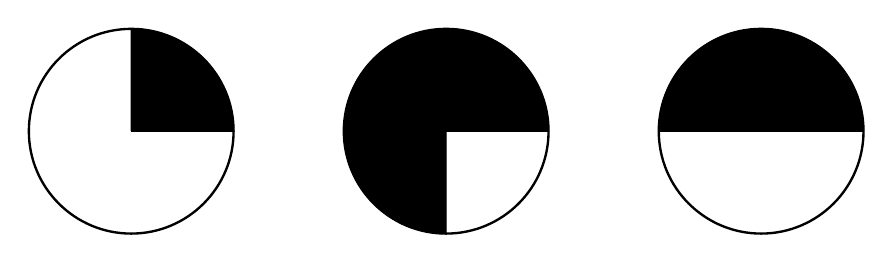
\begin{tikzpicture}
	\draw[line width=0.03cm] (0,0) circle (1.3);
	\draw[fill=black] (0,0) -- (1.3,0) arc[start angle=0, end angle=90,radius=1.3] -- (0,0);
	
	\draw[line width=0.03cm] (4,0) circle (1.3);
	\draw[fill=black] (4,0) -- (5.3,0) arc[start angle=0, end angle=270,radius=1.3] -- (4,0);

	\draw[line width=0.03cm] (8,0) circle (1.3);
	\draw[fill=black] (8,0) -- (9.3,0) arc[start angle=0, end angle=180,radius=1.3] -- (8,0);
	\end{tikzpicture} 
	\]
If you spin each of these three spinners, one after the other, what is the probability that each spinner lands in the dark shaded area?
	\begin{enumerate}[A.]
	\item $0.09375$
	\item $0.50000$
	\item $0.66667$
	\item $0.75000$
	\end{enumerate}

% Question 8
\question Let $S$ be the set of counting numbers from 1 to 100 (including 1 and 100). Suppose you found the mean, median, IQR, and standard deviation of $S$. Which of the following statements is most accurate if you were to compute these statistics after including the number 1,200 in the set $S$?
	\begin{enumerate}[A.]
	\item The mean would change more than the median.
	\item The median would change more than the mean.
	\item The mean and median would change by the same amount.
	\item The mean would change but the median would not.
	\end{enumerate}

% Question 9
\question Which of the following represents the region shaded in the Venn diagram below?
	\[
	\begin{venndiagram2sets}[tikzoptions={scale=1}]
	\fillOnlyA
	\end{venndiagram2sets}	
	\]
	
	\begin{enumerate}[A.]
	\item $A$
	\item $A \cap B$
	\item $A - B$
	\item $(A \cup B) - (A \cap B)$
	\end{enumerate}

% Question 10
\question Samantha, Timothy, Ben, and Justin are lining up at the cafeteria for lunch. How many arrangements are there for them to line up?
 	\begin{enumerate}[A.]
	\item 1
	\item 4
	\item 10
	\item 24
	\end{enumerate}

% Question 
\question Shown below is a spinner with different regions labeled, as well as the angles used to form those regions. \par
	\[
	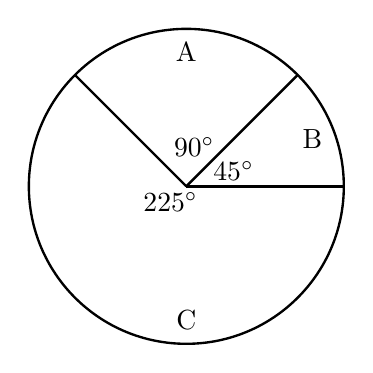
\begin{tikzpicture}
	\draw[line width=0.03cm] (0,0) circle (2);
	\draw[line width=0.03cm] (0,0) -- (2,0);
	\draw[line width=0.03cm] (0,0) -- (1.414,1.414);
	\draw[line width=0.03cm] (0,0) -- (-1.414,1.414);
	\node at (0,-1.7) {C};
	\node at (1.6,0.6) {B};
	\node at (0,1.7) {A};
	\node at (0.6,0.2) {$45^\circ$};
	\node at (0.1,0.5) {$90^\circ$};
	\node at (-0.2,-0.2) {$225^\circ$};
	\end{tikzpicture}
	\] \par
If you spin this wheel, what is the probability that the spinner lands in the region labeled `C'?
	\begin{enumerate}[A.]
	\item $\frac{1}{2}$
	\item $\frac{2}{3}$
	\item $\frac{5}{8}$
	\item $\frac{7}{8}$
	\end{enumerate}

% Question 
\question Below are box plots for the exam scores for students in a Mathematics class, broken down by gender. The women are represented by red and men by blue. \par
\begin{tikzpicture}
  \begin{axis}
    [
%    ytick={1,2}
	yticklabels={Men, Women}
    ]
    \addplot+[
    boxplot prepared={
      median=65,
      upper quartile=72,
      lower quartile=63,
      upper whisker=85.5,
      lower whisker=49.5
    },
    ] coordinates {};
    \addplot+[
    boxplot prepared={
      median=80,
      upper quartile=83,
      lower quartile=78,
      upper whisker=90.5,
      lower whisker=70.5
    },
    ] coordinates {};
  \end{axis}
\end{tikzpicture}
Which of the following statements is most accurate?
	\begin{enumerate}[(a)]
	\item On average, the women did better and the men had more varied scores.
	\item On average, the men did better and the women had more varied scores.
	\item On average, the women did better and the men had less varied scores. 
	\item On average, the men did better and the women had less varied scores. 
	\end{enumerate}

% Question 
\question Let $C$ be the set of cars, $O$ be the set of objects that were made more than five years ago, and $R$ be the set of red objects. Which of the following best describes an element of $(C \cap O^c) \cup (C \cap R)$?
	\begin{enumerate}[A.]
	\item A red car that was made more than 5 years ago.
	\item A red car that was made less than 5 years ago.
	\item A red car or a car made more than 5 years ago.
	\item A red car or a car made less than 5 years ago.
	\end{enumerate}

% Question 
\question How many passwords with 6~characters can be made using the first five letters of the alphabet and the numbers 0--4?
	\begin{enumerate}[A.]
	\item 10
	\item 531,441
	\item 1,000,000
	\item 3,628,800
	\end{enumerate}

% Question 
\question CHART PROB

% Question 
\question Which of the following would not be appropriate to use to represent the set of average monthly temperatures from January 2000 to December 2019?
	\begin{enumerate}[A.]
	\item A dot plot.
	\item A box plot.
	\item A stem-and-leaf plot.
	\item A histogram.
	\end{enumerate}

% Question 
\question Which of the following is the cardinality of the set of even numbers from 10 to 620 (including 0 and 100)?
	\begin{enumerate}[A.]
	\item 290
	\item 305
	\item 306
	\item 610
	\end{enumerate}

% Question 
\question 14.2, 15

% Question 
\question CHART PROB

% Question 
\question Robert calculates that, on average, they make \$47.50 in profit for each person that attends one of the baseball games at the stadium where he works. If there were 8,400 people that attended the last game, approximately how much profit did the stadium make?
	\begin{enumerate}[A.]
	\item \$8,400
	\item \$399,000
	\item \$420,000
	\item \$1,500,000
	\end{enumerate}

% Question 
\question If $A= \{ a, b, a, c, d, e \}$ and $B= \{ a, b, e, e \}$, which of the following is the set $A \cap B$?
	\begin{enumerate}[A.]
	\item $\{ a, a, b \}$
	\item $\{ a, b, e \}$
	\item $\{ a, a, b, d, e, e \}$
	\item None of the above
	\end{enumerate}

% Question 
\question What is the cardinality of the set $A= \{ 1, 1, 2, 2, 3, 3, \ldots, 10, 10 \}$?
	\begin{enumerate}[A.]
	\item 4
	\item 8
	\item 10
	\item 20
	\end{enumerate}
 

% Question 
\question 6 chart prob

% Question 
\question 6 which result/not in bias

% Question 
\question 7 cardinality set difference

% Question 
\question 6 comb 

% Question 
\question 7 venn prob

% Question 
\question 8 z-score special sections

% Question 
\question 8 complement of set in interval

% Question 
\question 8 perm 

% Question 
\question 9 dice prob roll

% Question 
\question 9 sketch normal which most likely mean stdev

% Question 
\question 5 cardinality of set with repeats 

% Question 
\question 7 comb

% Question 
\question 10 dice prob roll

% Question 
\question 10 which is outlier for data set (iqr)

% Question 
\question 9 whether element

% Question 
\question 9 perm

% Question 
\question 11 marble prob

% Question 
\question 12 add data value happens mean \& stdev

% Question 
\question Let $P$ be the set of all prime numbers and $O$ be the set of all odd numbers. Which of the following is true?
	\begin{enumerate}[A.]
	\item $P \subseteq O$
	\item $O \subseteq P$
	\item $P= O$
	\item $P \neq O$
	\end{enumerate}


% Question 
\question 10 random COUNT

% Question 
\question 8 ven prob

% Question 
\question 14 for data set which largest mean, med, mod, \#

% Question 
\question prob disjoint indep

% Question 
\question 11 which 5-number summary

% Question 
\question 15 chart problem

% Question 
\question 13 boxplot find mean iqr

% Question 
\question set

% Question 
\question other


\end{questions}
\end{document}